\documentclass[a4paper,10pt]{article} 
%\usepackage[style=nature,backend=biber]{biblatex}
\usepackage{graphicx}
\usepackage[font={it},labelfont={bf}]{caption}
\usepackage{times}
\usepackage{color}
%\usepackage{fixltx2e} % fixes placing of image positions
\usepackage{authblk}
\usepackage{amsmath}
\usepackage{courier}
\usepackage[round]{natbib}
\usepackage{wrapfig}

\definecolor{customhdrcolor}{rgb}{0.0,0.0,0.0}
%\definecolor{customcitecolor}{rgb}{0.0,0.25,0.25}
\definecolor{customcitecolor}{rgb}{0.0,0.5,0.75}
%\definecolor{customlinkcolor}{rgb}{0.0,0.0,1.0}
\definecolor{customlinkcolor}{rgb}{0.0,0.5,0.75}

\usepackage[colorlinks=true,linkcolor=customlinkcolor,urlcolor=customlinkcolor,citecolor=customcitecolor,pdftex]{hyperref}

\ifpdf\pdfinfo{/Title      (Report on D0002 observations: high spectral resolution RFI analysis)
               /Author     (A. R. Offringa)
               /Keywords   (MWA, RFI, spectral resolution)
        }
\else\usepackage{graphics}\fi

\setlength{\pdfpageheight}{\paperheight}
\setlength{\pdfpagewidth}{\paperwidth}

\title{Report on D0002 observations: high spectral resolution RFI analysis}

\author{A.~R.~Offringa}
%\author[1,2]{A.~R.~Offringa}
%\affil[1]{RSAA, Australian National University, Mt Stromlo Observatory, via Cotter Road, Weston, ACT 2611, Australia}
%\affil[2]{ARC Centre of Excellence for All-Sky Astrophysics (CAASTRO)}
\begin{document}

\label{firstpage}
\maketitle

\section{Goals}
MWA director's time was requested to compare RFI detection accuracy between a spectral resolution of 10~kHz and 40~kHz. High spectral resolution has been a major benefit for dealing with the RFI environment of LOFAR \citep{lofar-radio-environment}. Whether the data quality improves with higher resolution, caused by more accurate RFI detection, is relevant for optimizing future MWA observing configurations. Moreover, for future telescopes such as the SKA it is very interesting to see how frequency resolution relates to data quality, especially in the quiet radio environment of the MWA. 

\section{Observations}
I received one hour of MWA data observed with a spectral resolution of 10~kHz and temporal resolution of 2~s. The observations were recorded in the night of 30-31 July 2013. The EoR bands covering 139--200~MHz with centre coarse channels 121 and 145 were selected. The first 4~min were spent on calibrator 3C444, after which the quiet EoR0 field was observed for 1h. The bands were observed intermittently in blocks of 5~min.

\section{Results}
The observations were processed with the Cotter MWA preprocessing pipeline, which flags the data using the AOFlagger RFI detector. This detector uses combinatorial thresholding \citep{post-correlation-rfi-classification} and morphological detection \citep{scale-invariant-rank-operator}.
\begin{figure*}
\begin{center}
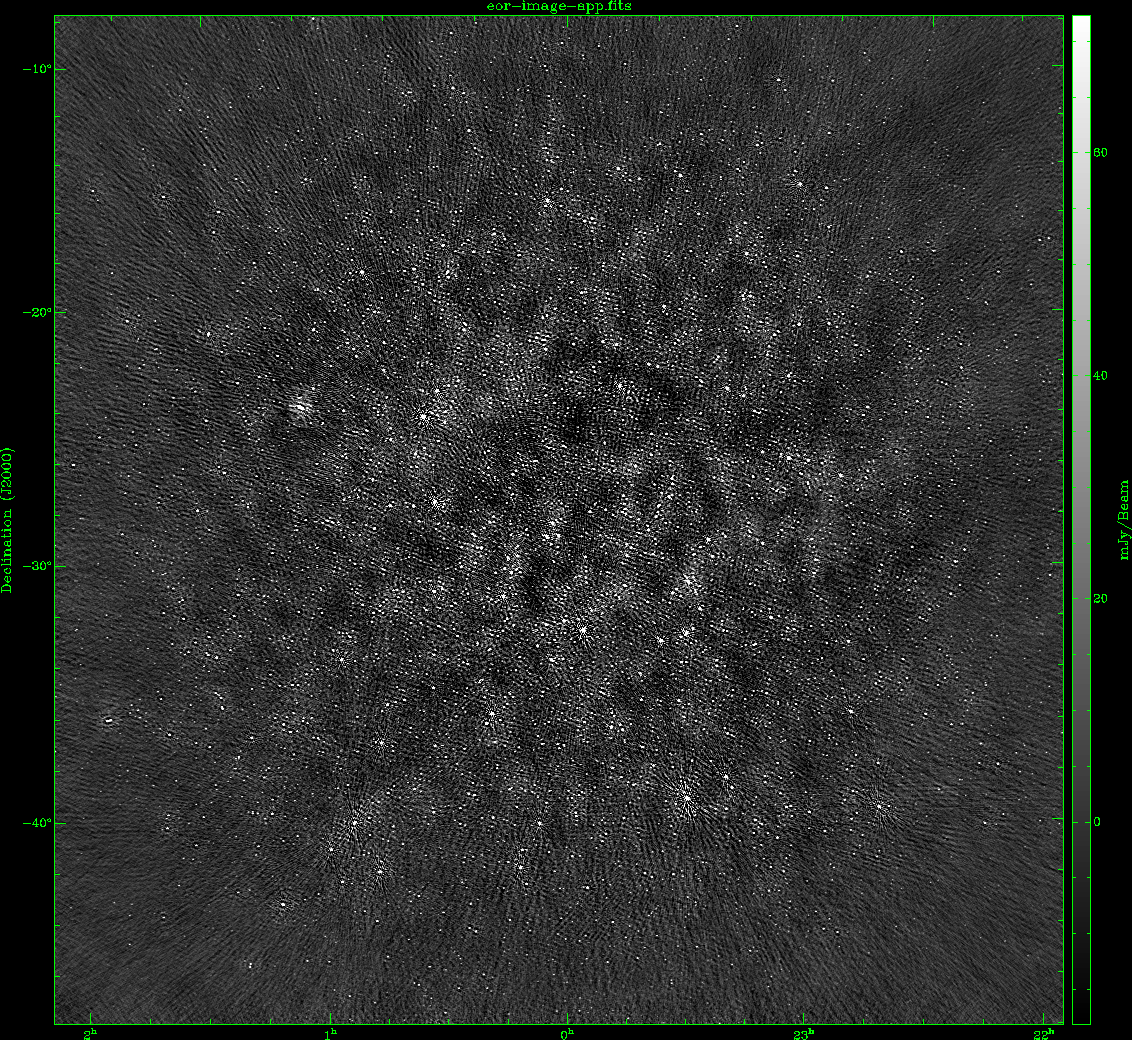
\includegraphics[width=12.5cm]{Apparent-image-EoR0.png}
\caption{Apparent image with 16 mJy noise level, deconvolved with {\tt wsclean}. These are the data after initial transfer of calibration solutions: no self-calibration or peeling has been applied yet. I believe it is the deepest MWA image made so far. Artefacts around the brightest sources are considerably decreased by self-calibration, but I have not made a deconvolved image of the self-calibrated data yet.}
\label{fig:eor0}
\end{center}
\end{figure*}
\subsection{Imaging quality}
The observations are of good quality. The calibrator scans are calibrated with a 3C444 point source model without any problems. A full polarization calibration script developed for the spectral analysis of sources in the EoR fields was used to do this. Transferring the 3C444 solutions to the EoR0 observations results in a reasonably good initial calibration. A resulting image of this is given in Fig.~\ref{fig:eor0}. Self-calibration and peeling increases the image quality further, but I have not made a deconvolved image with all data after self-calibration and peeling. Imaging only half the data results in an increase of noise very close to $\sqrt{2}$, suggesting that the observation is not yet confusion limited. The noise level is not as deep as estimated by $t \approx 8 \times 10^4/B\sigma^2_s$, formula (4) in \citet{mwa}. That formula results in $\sigma = 0.89$ mJy for an hour of data (with $B=30.72$~MHz~$\times 22/24$ due to the missing GPU boxes), which is a factor of $\sim 18$ lower than the actually observed noise level. This deficient might be partially caused by calibration artefacts, but further self-calibration and peeling did not decrease the noise more than a few mJy. This is a quiet field, so one should expect that any field will need more time (and calibration effort) to reach the desired noise limit. It seems unlikely that RFI is the cause of this deficiency.

\subsection{RFI analysis}
\begin{wraptable}{r}{6cm}
\caption{List of most dominant RFI sources in the range 139--200 MHz. Occupancy values describe the ratio of detected RFI in a 10 kHz channel over the full hour.}\label{table:rfi-sources}\begin{center}\begin{tabular}{rrr}
\hline
\hline
\textbf{Frequency}& \textbf{Occupancy} & \textbf{Coarse ch} \\
\textbf{(MHz)}& \textbf{(\%)} & \textbf{number} \\
\hline
141.685 &  0.97 & 111 \\
145.955 &  8.01 & 114 \\
149.955 & 31.52 & 117 \\
150.025 & 29.96 & 117 \\
178.745 &  4.13 & 140 \\
186.155 &  1.88 & 145 \\
194.455 &  2.02 & 152 \\
200.015 &  6.15 & 156 \\
\hline
\end{tabular}
\end{center}
\end{wraptable}

\begin{figure*}
\begin{center}
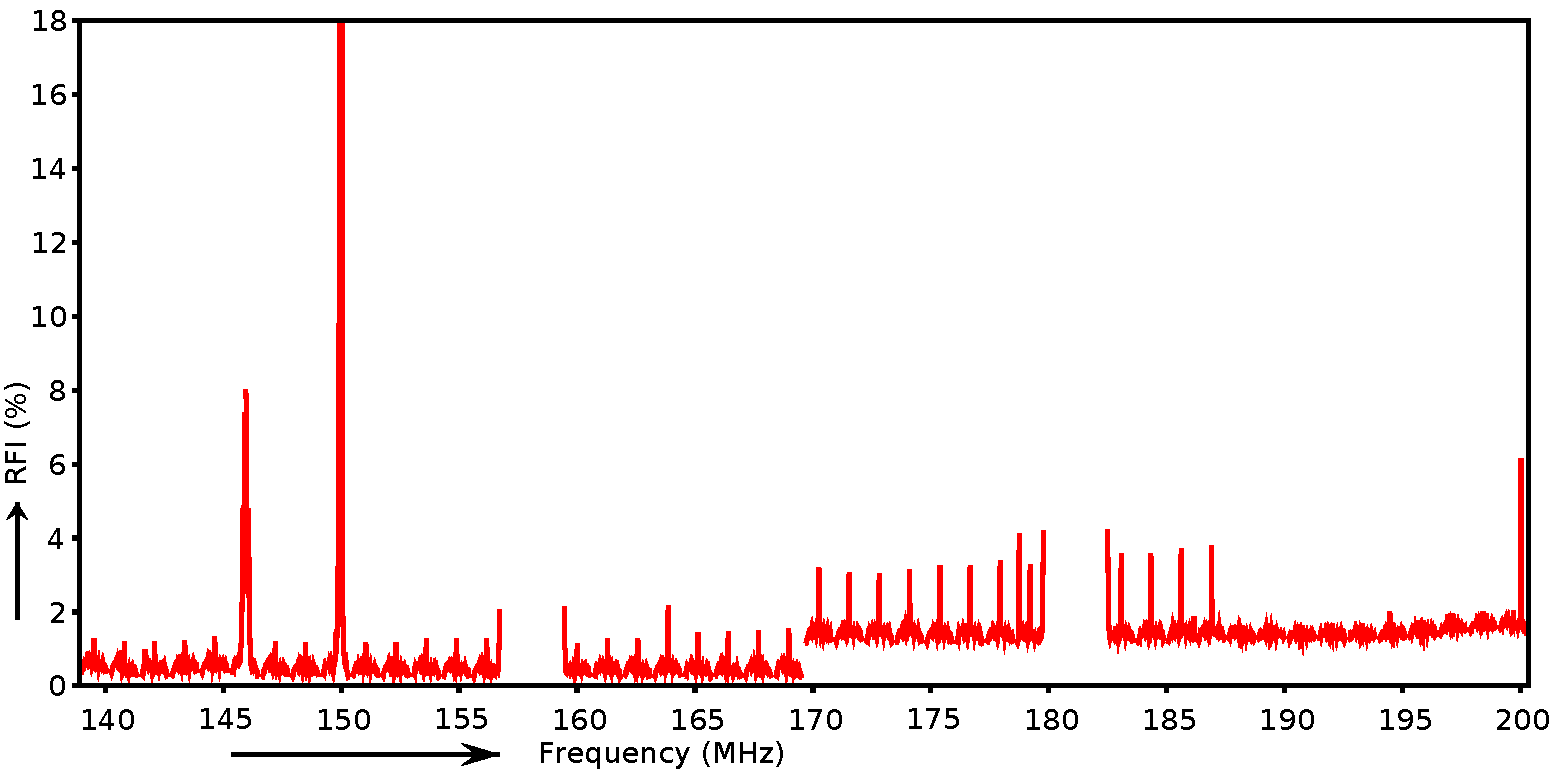
\includegraphics[width=12cm]{rfi-spectrum.pdf}
\caption{Detected RFI ratio over frequency for all visibilities (1~h, all correlations). The visible transmitters are enumerated in Table~\ref{table:rfi-sources}. The gaps around 157 and 181~MHz are because of two broken GPU correlator boxes. The 1.28~MHz periodic structure is because of the poly-phase filter: each 1.28 MHz sub-band represents a coarse channel. }
\label{fig:rfi-spectrum}
\end{center}
\end{figure*}

The amount of RFI in these observations is relatively low -- lower than previously observed in a South Galactic Pole RFI measurement with 32T. This might be because of a different sensitivity towards the horizon due to different beam former settings, but it could also be accidental. The RFI environment in more recent EoR1 observations looks similar to these EoR0 observations. The strongest RFI contaminator with the MWA band comes from the Orbcom satellites, but these transmit outside the bandwidth of these observations. Fig.~\ref{fig:rfi-spectrum} shows the amount of detected RFI over frequency, for the full hour. Two transmitters around 146 and 150 MHz are clearly visible, but a few more can be identified. The signal at 150 MHz seems to contaminate two channels that are 70 kHz apart, so this signal could come from two transmitters. A list of channels containing a significant amount of RFI are listed in Table~\ref{table:rfi-sources}. There are a few more peaks in the data, but it is hard to distinguish the DC channel offset problem and coarse channel edges from actual low-level RFI contamination. 

\begin{figure*}
\begin{center}
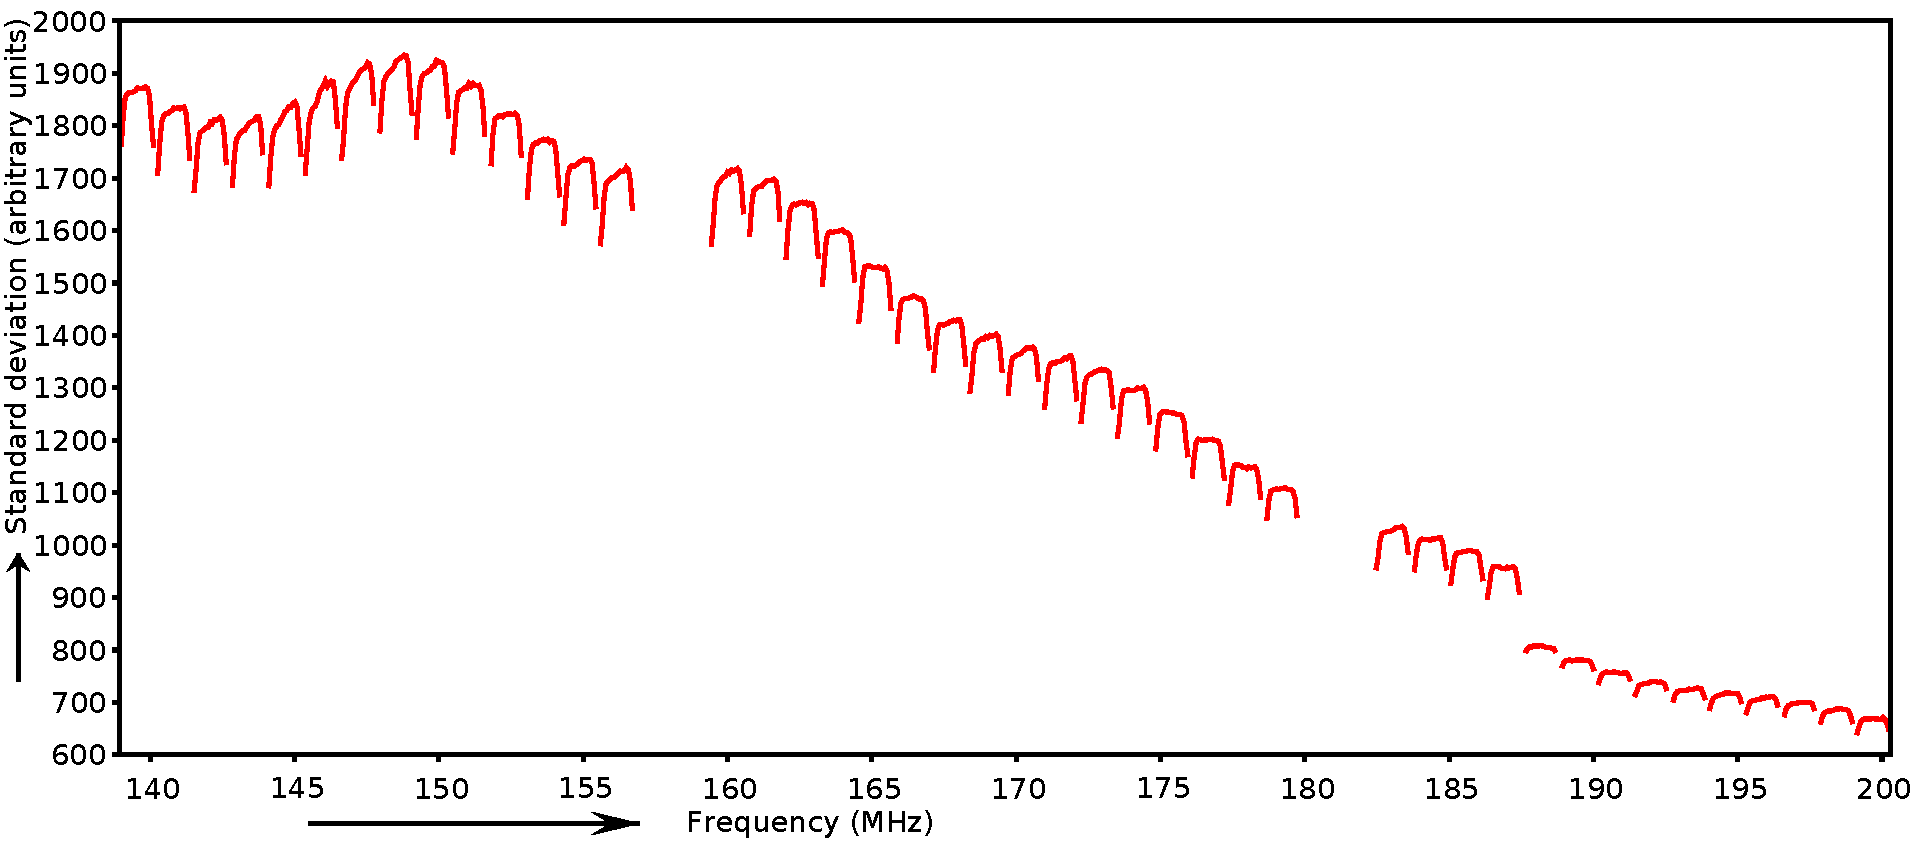
\includegraphics[width=12cm]{stddev-spectrum.pdf}
\caption{Standard deviation over frequency for all visibilities (1~h, all correlations). No significant RFI residuals are visible. The jump at 187~MHz is because of digital gains that are applied to the data before correlation, resulting in different noise statistics.}
\label{fig:stddev-spectrum}
\end{center}
\end{figure*}

The flagger performs an accurate rejection and flags almost all RFI. At 10 kHz, 0.83\% of all data is lost due to RFI. Fig.~\ref{fig:stddev-spectrum} shows the standard deviation of all the data after the RFI rejection. There is a small noise increase around 147 MHz. To see how much frequency resolution affects the quality, I have averaged the data to 40~kHz and reapplied the AOFlagger. The resulting standard deviation plot looks extremely similar. The only difference is that at 40 kHz the amount of detected RFI is about 1\% higher. This is hard to estimate accurately using these data, because of the DC channel and sideband edges that get into the statistics. Cotter makes sure to keep these out of the statistics, but a standalone run of the AOFlagger is required to flag the 40 kHz data, and the AOFlagger does not distinguish between DC channels and RFI. On EoR1 data, typical RFI occupancies reported by Cotter are $\sim 1.65$\%, agreeing with the fact that at 40 kHz about 1\% more data is lost due to RFI.

\subsection{Other uses of these observations}
\begin{itemize}
 \item Undergraduate student Jake Hughes has used these data to analyze whether RFI events can be located to a specific point on the sky (or horizon). Certain constant transmitters were clearly visible as peaks in the sky when the data was not flagged. He also tried to image short bursts of RFI, that were apparent in a few time steps. These only increased the noise in the image, but this affected the whole sky image, and not a specific part of the sky. It is likely that these RFI burst are therefore occurring in the near field.
 \item Because of its high quality, I have used these data extensively to develop my spectral analysis software.
 \item I have provided the observations with self-calibration and subtraction of the brightest sources to Cathryn Trott, who will use these to test her EoR pipeline.
 \item The observations can be included in the other EoR analyses.
\end{itemize}
The latter three items do of course not necessarily require the high spectral resolution. However, clearly these observations have been used extensively and were very helpful.

\section{Conclusions}
\begin{itemize}
 \item The observations were of high quality.
 \item The image noise is more than an order of magnitude worse than estimated by \citet{mwa}. Some improvement might be made by spending more effort on calibration, but I think the formula given by Tingay et al. is too optimistic.
 \item RFI is not much of a concern for MWA in the 139--200~MHz frequency range. About 1.65\% is lost due to RFI at 40~kHz, while 0.83\% is lost at 10~kHz. In general no leaked RFI is visible after applying the AOFlagger. That does not necessarily mean there is none, but it seems to be insignificant from current data.
 \item Preliminary, the only benefit that 10~kHz observations seems to have on RFI rejection, is that about 1\% less data is lost due to RFI. This should be tested at different beam former settings, different epochs and different frequencies to make sure this is the case in general.
 \item We now have a baseline of RFI measurements, which will be useful to compare to in the future. Regularly repeating such a test will be useful.
\end{itemize}

\label{lastpage}

\bibliographystyle{plainnat}
\bibliography{references}

\end{document}
